\documentclass[11pt]{article}
\usepackage{listings}
\usepackage{graphicx}
\newcommand{\numpy}{{\tt numpy}}    % tt font for numpy

\topmargin -.5in
\textheight 9in
\oddsidemargin -.25in
\evensidemargin -.25in
\textwidth 7in

\begin{document}

% ========== Edit your name here
\author{Francesco Penasa}
\title{Distributed System 1 - synch 5}
\maketitle

\medskip

% ========== Begin answering questions here
\texttt{2020 03 09}
\section{Examples} % (fold)
\label{sec:examples}
\subsection{synch} % (fold)
\label{sub:synch}

Simple Logical Clock
\begin{figure}[ht]
	\centering
	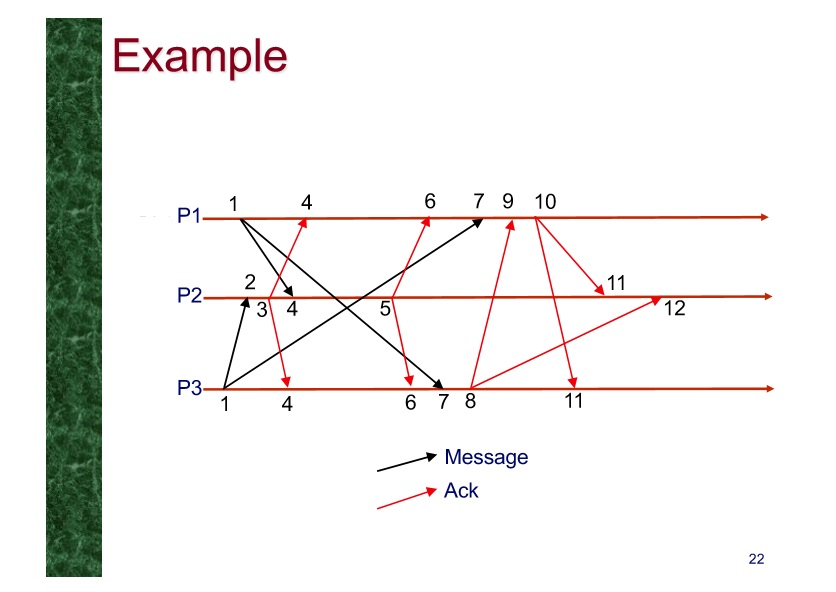
\includegraphics[scale=0.5]{figures/example_synch_1.jpg}
	\caption{Logical Clock}
	\label{fig:logical}
\end{figure}

\subsubsection{Distributed Snapshot} % (fold)
\label{ssub:distributed_snapshot}
\paragraph{Distributed Snapshot algorithm} % (fold)
\label{par:distributed_snapshot_algorithm}
Chandy-Lamport, 1985
% paragraph distributed_snapshot_algorithm (end)
\begin{enumerate}
	\item Assume FIFO, reliable links/nodes, strongly connected graph.
	\item Any process can initiate a snapshot by
	\begin{enumerate}
		\item Recording internal state
		\item Sending a token on all outgoing channels
		\item Start recording local snapshot (record messages arriving on every incoming channel).
	\end{enumerate}
	\item Upon receiving a token
	\begin{enumerate}
		\item if not already recording local snapshot, initiate the snapshot (2a, 2b and 2c).
		\item in any case stop recording incoming message on channel the token arrived along. 
	\end{enumerate}
	\item Recording messages
	\begin{enumerate}
		\item If a message arrives on a channel which is recording messages, record the arrival of the message, then process the message as normal.
		\item Otherwise, just porcess the message as normal.
	\end{enumerate}
	\item Snapshot complete when token has arrived on all incoming channels.
	\begin{enumerate}
		\item Irrelevant how the various data arec collected and/or transmitted.
	\end{enumerate}
\end{enumerate}
% subsubsection distributed_snapshot (end)

% subsection synch (end)
% section examples (end)
\section{Exercises} % (fold)
\label{sec:exercises}

\subsection{synch} % (fold)
\label{sub:synch}
\subsubsection{Logical Clock} % (fold)
\label{ssub:logical_clock}

% subsubsection logical_clock (end)\
\subsubsection{Distributed Snapshot} % (fold)
\label{ssub:distributed_snapshot}
\paragraph{ex1} % (fold)
\label{par:ex1}
% paragraph ex1 (end)
\begin{figure}[ht]
	\centering
	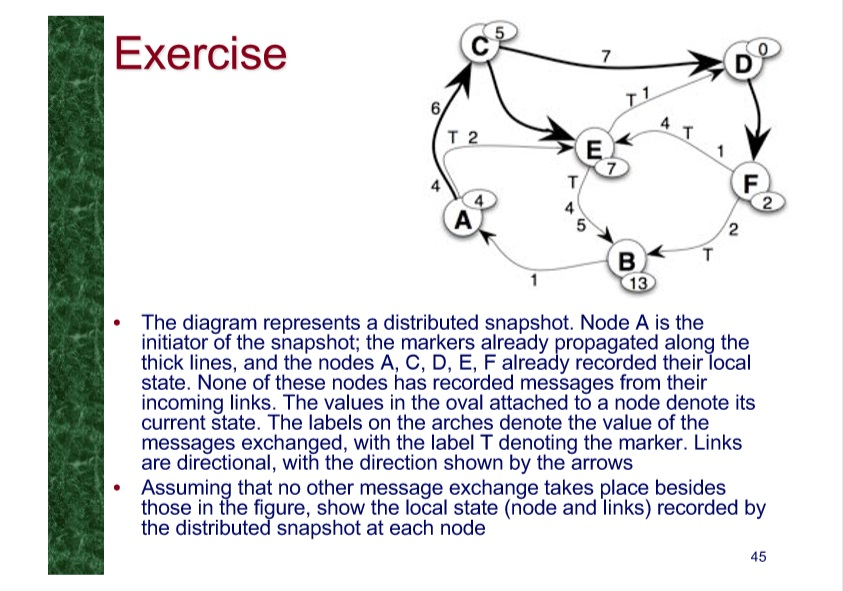
\includegraphics[scale=0.7]{figures/exercise_synch_3.jpg}
	\caption{Distributed Snapshot Exercise 1}
	\label{fig:dse1}
\end{figure}
\begin{enumerate}
	\item A 15
	\item B 22
	\item C 12
	\item D 1
	\item E 13
	\item F 5
\end{enumerate}

\paragraph{ex 2} % (fold)
\label{par:ex_2}
\begin{figure}[ht]
	\centering
	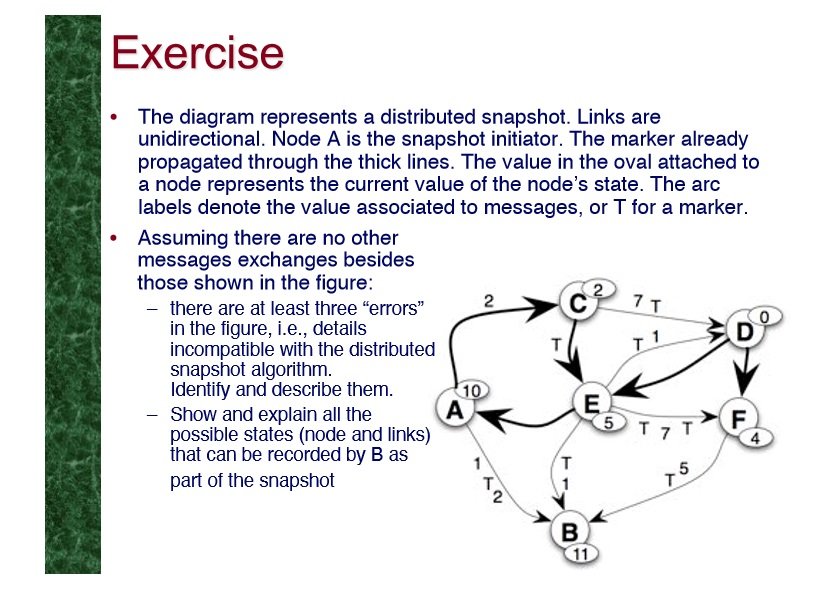
\includegraphics[scale=0.7]{figures/exercise_synch_4.jpg}
	\caption{Distributed Snapshot Exercise 2}
	\label{fig:dse2}
\end{figure}
\begin{enumerate}
	\item C to E has a T even if it is an already marked link
	\item E to F: there are two T on the same unidirectional link.
	\item D to E and D to F: can't have been happened if A was the initiator since D has to receive a mark from anyone before starting sending marks.
\end{enumerate}
B could record all the states but not all the links (not clear question)
% paragraph ex_2 (end)
% subsubsection distributed_snapshot (end)
% subsection synch (end)

% section exercises (end)

\end{document}
\grid
\grid